% -----------------------------------------------------------------------
% Section: Results (Phase 1 — Re=10 unsteady flow)
% -----------------------------------------------------------------------

\subsection{Reference Solution}

The reference solution is generated by a Chorin fractional-step
projection method~\cite{chorin1968projection} on a
uniform $220\times82$ grid with time step $\Delta t = 0.001$~s over the
interval $t\in[0,\,0.5]$~s, yielding 51 snapshots at $\Delta t_\text{snap}
= 0.01$~s.  The physical parameters and boundary conditions match those
described in Section~III exactly.

\subsection{Quantitative Error Comparison}

The $L_2$ relative error is defined as
\begin{equation}
  \varepsilon = \frac{\|\mathbf{u}_\text{pred} - \mathbf{u}_\text{ref}\|_F}
                     {\|\mathbf{u}_\text{ref}\|_F},
  \label{eq:l2rel}
\end{equation}
where $\|\cdot\|_F$ denotes the Frobenius norm over all grid points at a
given snapshot.  Errors are evaluated over the 41 snapshots with
$t\geq0.1$~s to exclude the initial transient during which the solution
magnitude is near zero.

The original Rao et al.~\cite{rao2020pinnflow} implementation cannot be
faithfully reproduced post-hoc---only a trained TensorFlow checkpoint is
available, and its training conditions cannot be exactly recovered.  We
therefore use our strict re-implementation of the Rao et al.\ protocol
with SciPy L-BFGS-B, denoted \emph{reproduce}, as the baseline, and
compare it against the \emph{GPU-resident} PyTorch variant whose L-BFGS
loop runs entirely on the GPU via \texttt{torch.optim.LBFGS}.  Both are
evaluated against the same Chorin CFD solution;
Table~\ref{tab:l2_snapshots} reports only relative errors, not
reference-field values.

\begin{table}[t]
  \caption{Per-snapshot $L_2$ relative error (\%) for $u$, $v$, and
           spatially demeaned $p$, $Re=10$.  \emph{reproduce} is the
           SciPy L-BFGS-B baseline; \emph{GPU-resident} is the PyTorch
           L-BFGS run.  Selected snapshots shown; best per column in bold.}
  \label{tab:l2_snapshots}
  \centering
  \resizebox{\columnwidth}{!}{%
  \begin{tabular}{@{}c ccc ccc@{}}
    \toprule
    & \multicolumn{3}{c}{reproduce} & \multicolumn{3}{c}{GPU-resident} \\
    \cmidrule(lr){2-4}\cmidrule(lr){5-7}
    $t$ (s) & $\varepsilon_u$ & $\varepsilon_v$ & $\varepsilon_p$
            & $\varepsilon_u$ & $\varepsilon_v$ & $\varepsilon_p$ \\
    \midrule
    0.10 & 10.19 & 41.74 &  3.44 & 11.87 & 47.50 &  2.42 \\
    0.20 &  5.63 & 24.39 &  4.29 &  6.77 & 27.27 &  4.23 \\
    0.30 &  4.25 & 16.47 &  9.06 &  4.93 & 18.61 &  9.04 \\
    0.40 &  4.44 & 13.29 &  4.45 &  4.50 & 14.70 &  6.33 \\
    0.50 &  4.81 & 12.60 & 70.08 &  4.72 & 13.57 & 63.86 \\
    \midrule
    Mean & \textbf{5.30} & \textbf{19.86} & 10.79 & 5.94 & 22.23 & \textbf{10.31} \\
    \bottomrule
  \end{tabular}}
\end{table}

\subsection{Discussion}

The \emph{GPU-resident} variant attains accuracy close to the
\emph{reproduce} baseline: the mean-error gap is $0.64$ percentage points in
$\varepsilon_u$ ($5.94\%$ vs.\ $5.30\%$) and $2.37$ points in
$\varepsilon_v$ ($22.23\%$ vs.\ $19.86\%$).  This gap is attributed to the
different L-BFGS backends---SciPy L-BFGS-B for \emph{reproduce}
versus PyTorch's native GPU \texttt{LBFGS} for \emph{GPU-resident}, which differ
in line search and stopping behaviour---together with minor random-seed
and collocation-sampling differences.  The GPU-resident loop keeps all
optimizer state on the GPU and avoids the per-evaluation host--device
transfer that the SciPy wrapper incurs on every function evaluation.

To isolate this effect we ran a controlled benchmark: starting from a
common Adam checkpoint, $1000$ L-BFGS function evaluations on the same
RTX~3090, varying \emph{only} the backend (SciPy L-BFGS-B versus
PyTorch's native GPU \texttt{LBFGS}).  Table~\ref{tab:backend_bench} and
Fig.~\ref{fig:backend_bench} summarize the result.  The GPU-resident
backend completes the $1000$ evaluations in $166$~s versus $204$~s for
SciPy ($1.23\times$ faster), reduces per-evaluation latency by $18.6\%$,
and increases mean GPU utilization from $68\%$ to $82\%$.  Although its
instantaneous GPU draw is higher, the shorter runtime lowers the
estimated benchmark energy from $59.8$ to $53.2$~kJ.  The SciPy wrapper
runs its L-BFGS-B linear algebra on the host and copies parameters and
gradients between device and host on every evaluation, whereas the
GPU-resident loop keeps optimizer state on the GPU.  The per-evaluation
floating-point work is identical, so the measured gap is backend
overhead; its magnitude is specific to this network size, collocation
count, and hardware.

\begin{table}[t]
  \centering
  \caption{Backend benchmark: $1000$ L-BFGS function evaluations from a
           common Adam checkpoint on one RTX~3090, $Re=10$.  Only the
           L-BFGS backend differs.  Energy is estimated as mean GPU draw
           multiplied by wall-clock time.}
  \label{tab:backend_bench}
  \footnotesize
  \setlength{\tabcolsep}{3.2pt}
  \begin{tabular}{@{}lccc@{}}
    \toprule
    Metric & reproduce & GPU-resident & Change \\
    \midrule
    Wall time       & $204.1$\,s & $\mathbf{166.4}$\,s & $1.23\times$ faster \\
    Eval latency    & $204$\,ms  & $\mathbf{166}$\,ms  & $18.6\%$ lower \\
    Energy          & $59.8$\,kJ & $\mathbf{53.2}$\,kJ & $11.0\%$ lower \\
    GPU utilization & $68\%$     & $\mathbf{82\%}$     & $+14$ pp \\
    \bottomrule
  \end{tabular}
\end{table}

\begin{figure}[t]
  \centering
  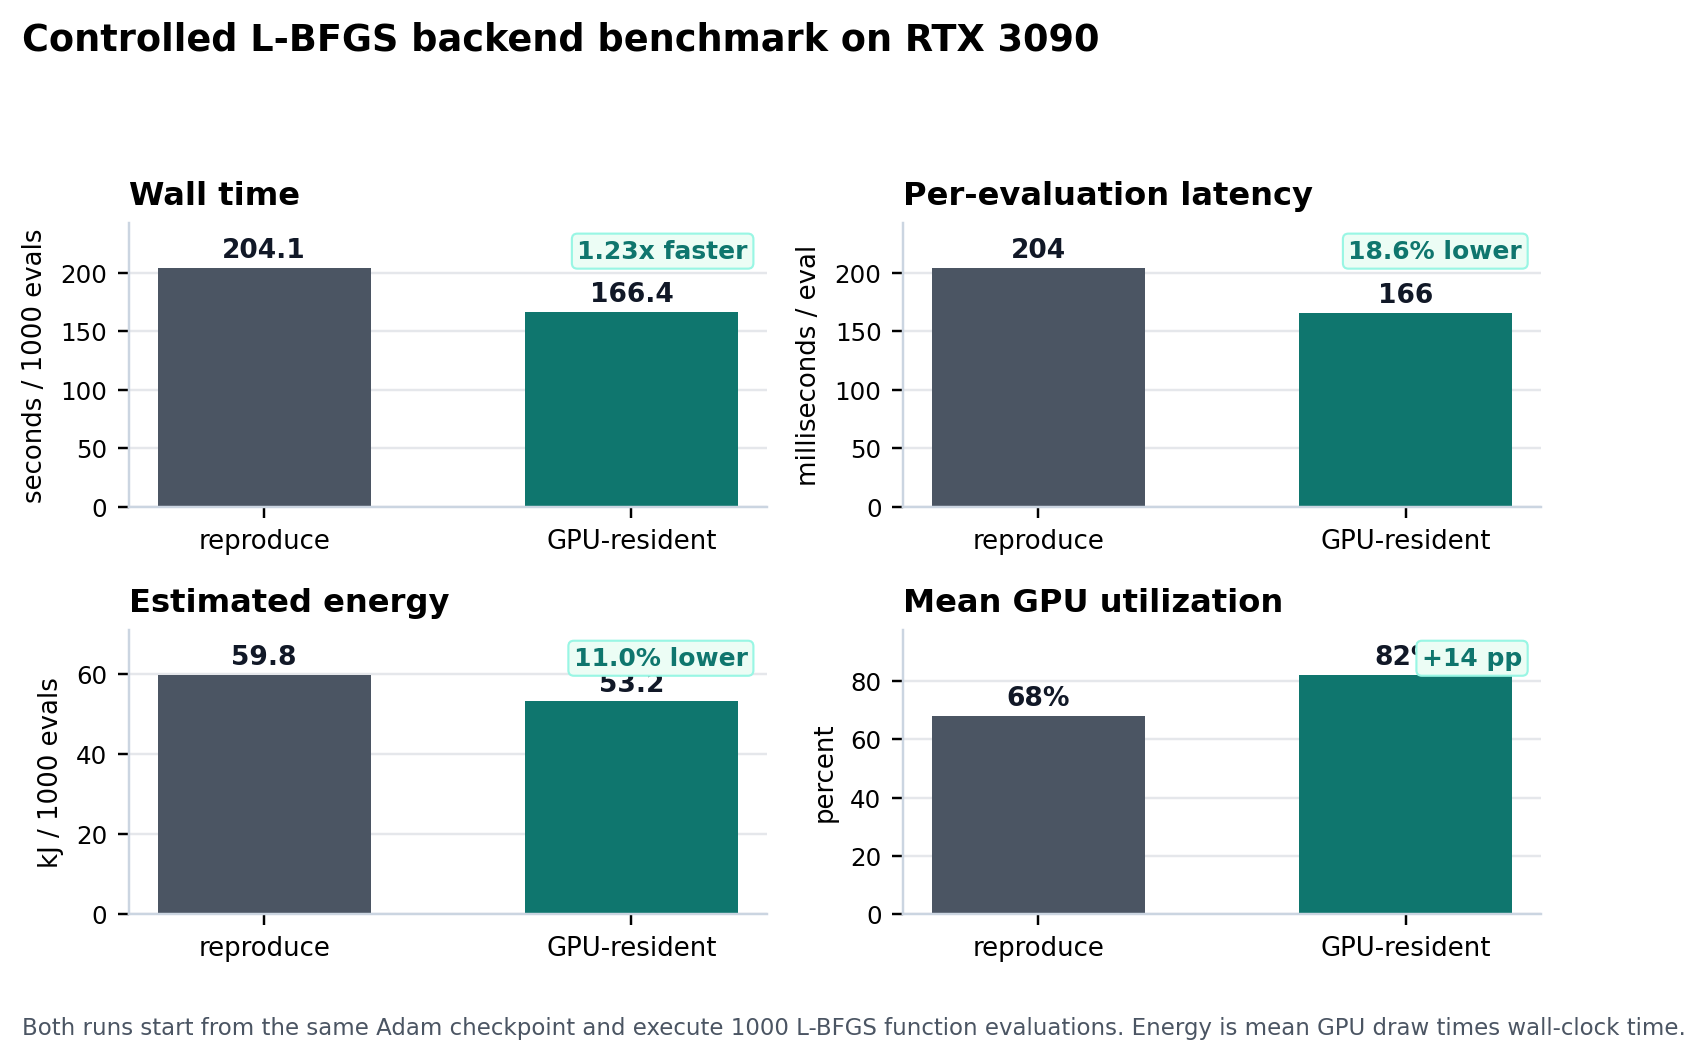
\includegraphics[width=\linewidth]{figures/lbfgs_backend_benchmark.png}
  \caption{Controlled backend comparison for $1000$ L-BFGS evaluations.
           The GPU-resident backend reduces wall-clock time, per-evaluation
           latency, and estimated energy while increasing mean GPU
           utilization.}
  \label{fig:backend_bench}
\end{figure}

The early-time snapshots ($t=0.10$--$0.20$~s) exhibit elevated errors
in both methods because the pulsatile inlet imposes the most rapid
variation; the PINN must satisfy a stiff constraint between the initial
condition ($u=v=0$ at $t=0$) and the imposed inlet profile, which is a
known source of difficulty for time-domain PINNs~\cite{wang2024causal}.

Pressure error is included after spatial demeaning to remove the arbitrary
pressure gauge.  The mean pressure errors are comparable
($10.79\%$ for \emph{reproduce} and $10.31\%$ for
\emph{GPU-resident}), although the final snapshot has a large pressure error
in both runs.  We therefore use pressure as a secondary diagnostic rather
than as the primary ranking criterion.

\todo{fig: field comparison of u, v, p at t=0.3, 0.4, 0.5 s for
GPU-resident vs reproduce vs Chorin reference (rainbow colormap, cylinder masked)}
